%%%%%%%%%%%%%%%%%%%%%%%%%
%% Header for standard beamer presentation
%%
%%  PresentationHeader.tex
%%
%%%%%%%%%%%%%%%%%%%%%%%%%

\documentclass[english,10pt]{beamer}

%%%%%%%%%%%%%%%%%%%%
%% Include general header where common packages are defined
%%%%%%%%%%%%%%%%%%%%

% general packages without options
\usepackage{amsmath,amssymb,bbm}




%%%%%%%%%%%%%%%%%%%%
%% Idem general commands
%%%%%%%%%%%%%%%%%%%%

%%% Commands

\newcommand{\noun}[1]{\textsc{#1}}


%% Math

% Operators
\DeclareMathOperator{\Cov}{Cov}
\DeclareMathOperator{\Var}{Var}
\DeclareMathOperator{\E}{\mathbb{E}}
\DeclareMathOperator{\Proba}{\mathbb{P}}

\newcommand{\Covb}[2]{\ensuremath{\Cov\!\left[#1,#2\right]}}
\newcommand{\Eb}[1]{\ensuremath{\E\!\left[#1\right]}}
\newcommand{\Pb}[1]{\ensuremath{\Proba\!\left[#1\right]}}
\newcommand{\Varb}[1]{\ensuremath{\Var\!\left[#1\right]}}

% norm
\newcommand{\norm}[1]{\| #1 \|}


% amsthm environments
\newtheorem{definition}{Definition}



%% graphics

% renew graphics command for relative path providment only ?
%\renewcommand{\includegraphics[]{}}






\usetheme{Warsaw}

\setbeamertemplate{footline}[text line]{}
\setbeamercolor{structure}{fg=purple!50!blue, bg=purple!50!blue}

\setbeamercovered{transparent}


% shortened command for a justified frame
\newcommand{\jframe}[2]{\frame{\frametitle{#1}\justify{#2}}}



%%%%%%%%%%%%%%%%%%%%%
%% Begin doc
%%%%%%%%%%%%%%%%%%%%%

\begin{document}



\title{Thesis Progress Meeting}


\author{J.~Raimbault$^{1,2}$}

\institute{$^{1}$G{\'e}ographie-Cit{\'e}s (UMR 8504 CNRS)\\
$^{2}$LVMT (UMR-T 9403 IFSTTAR)}


\date{July 2th 2015
}


%%%%%%%%%%%%%%%%%%%%%%%%%%%%%%%%
\begin{frame}
\titlepage
\end{frame}

%\begin{frame}
%\tableofcontents
%\end{frame}
%%%%%%%%%%%%%%%%%%%%%%%%%%%%%%%%


\section{Projects Organization}

%\jframe{Projects Organization}{
%   \includegraphics[width=\textwidth,height=0.8\textheight]{figures/orgaProjects}
%}



\section{Achieved Work}


\jframe{Achieved Work (by projects)}{
\begin{itemize}
\item Conference ICCSS :
\begin{itemize}
\item Conference [1w]
\item Bibliography [0.4w]
\item Poster preparation [0.4w]
\end{itemize}
\item MetropolSim model : Operational version ; first exploration. [1w]
\item Space Matters project : coding of morphological indicators and generative models into scala model. [0.4w]
\item Network-density statistics : fine systematic study of european urban morphology ; preparation of NW data (direct OSM import). [0.6w]
\item Synthetic Data Control : formalisation of the approach. [0.4w]
\end{itemize}
}



\section{Technical Developments}





%%%%%%%%%%%%%%%%%%%%%%%%%%%%%%%%
\jframe{MetropolSim Model : first exploration results}{
\hspace{-1cm}
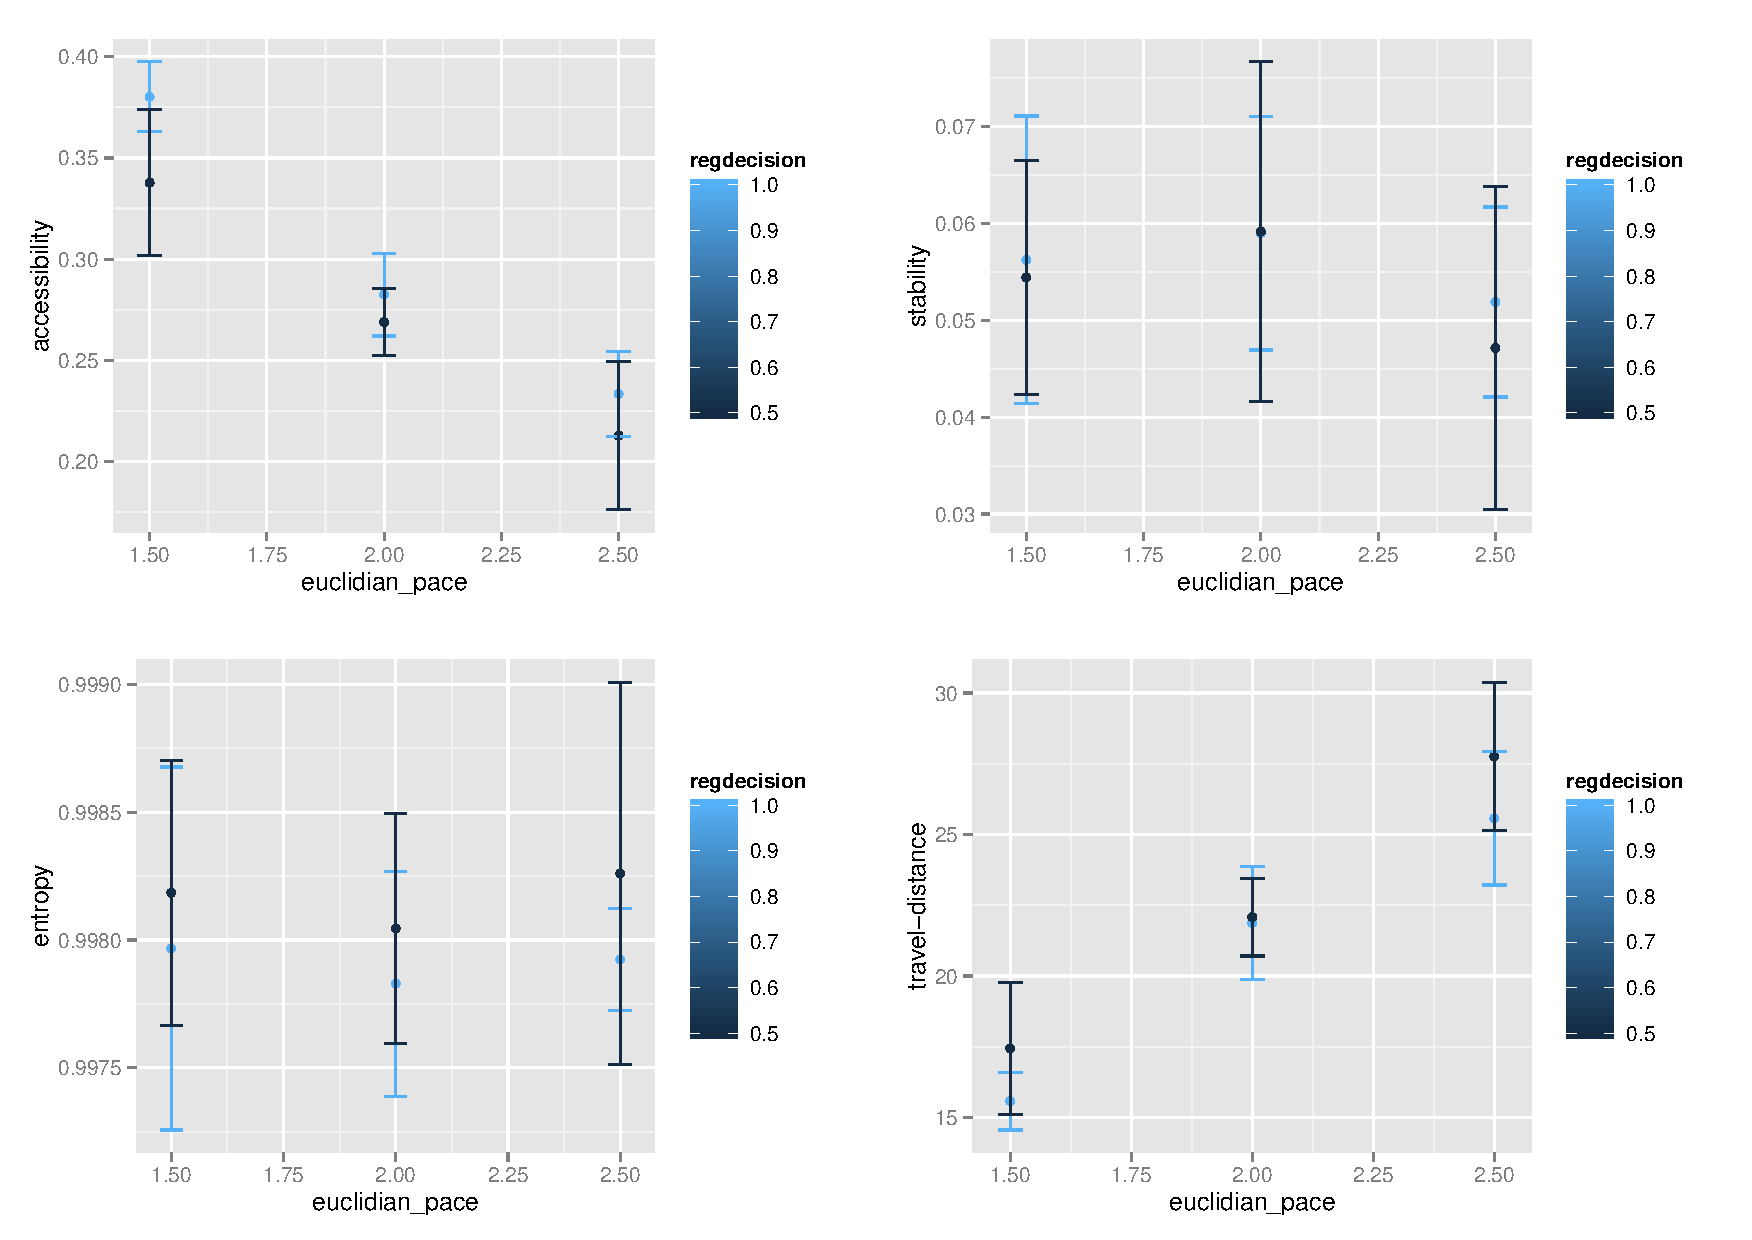
\includegraphics[width=0.6\textwidth,height=0.8\textheight]{figures/allIndics_euclPaceVarying_lambdaAcc=0075.pdf}
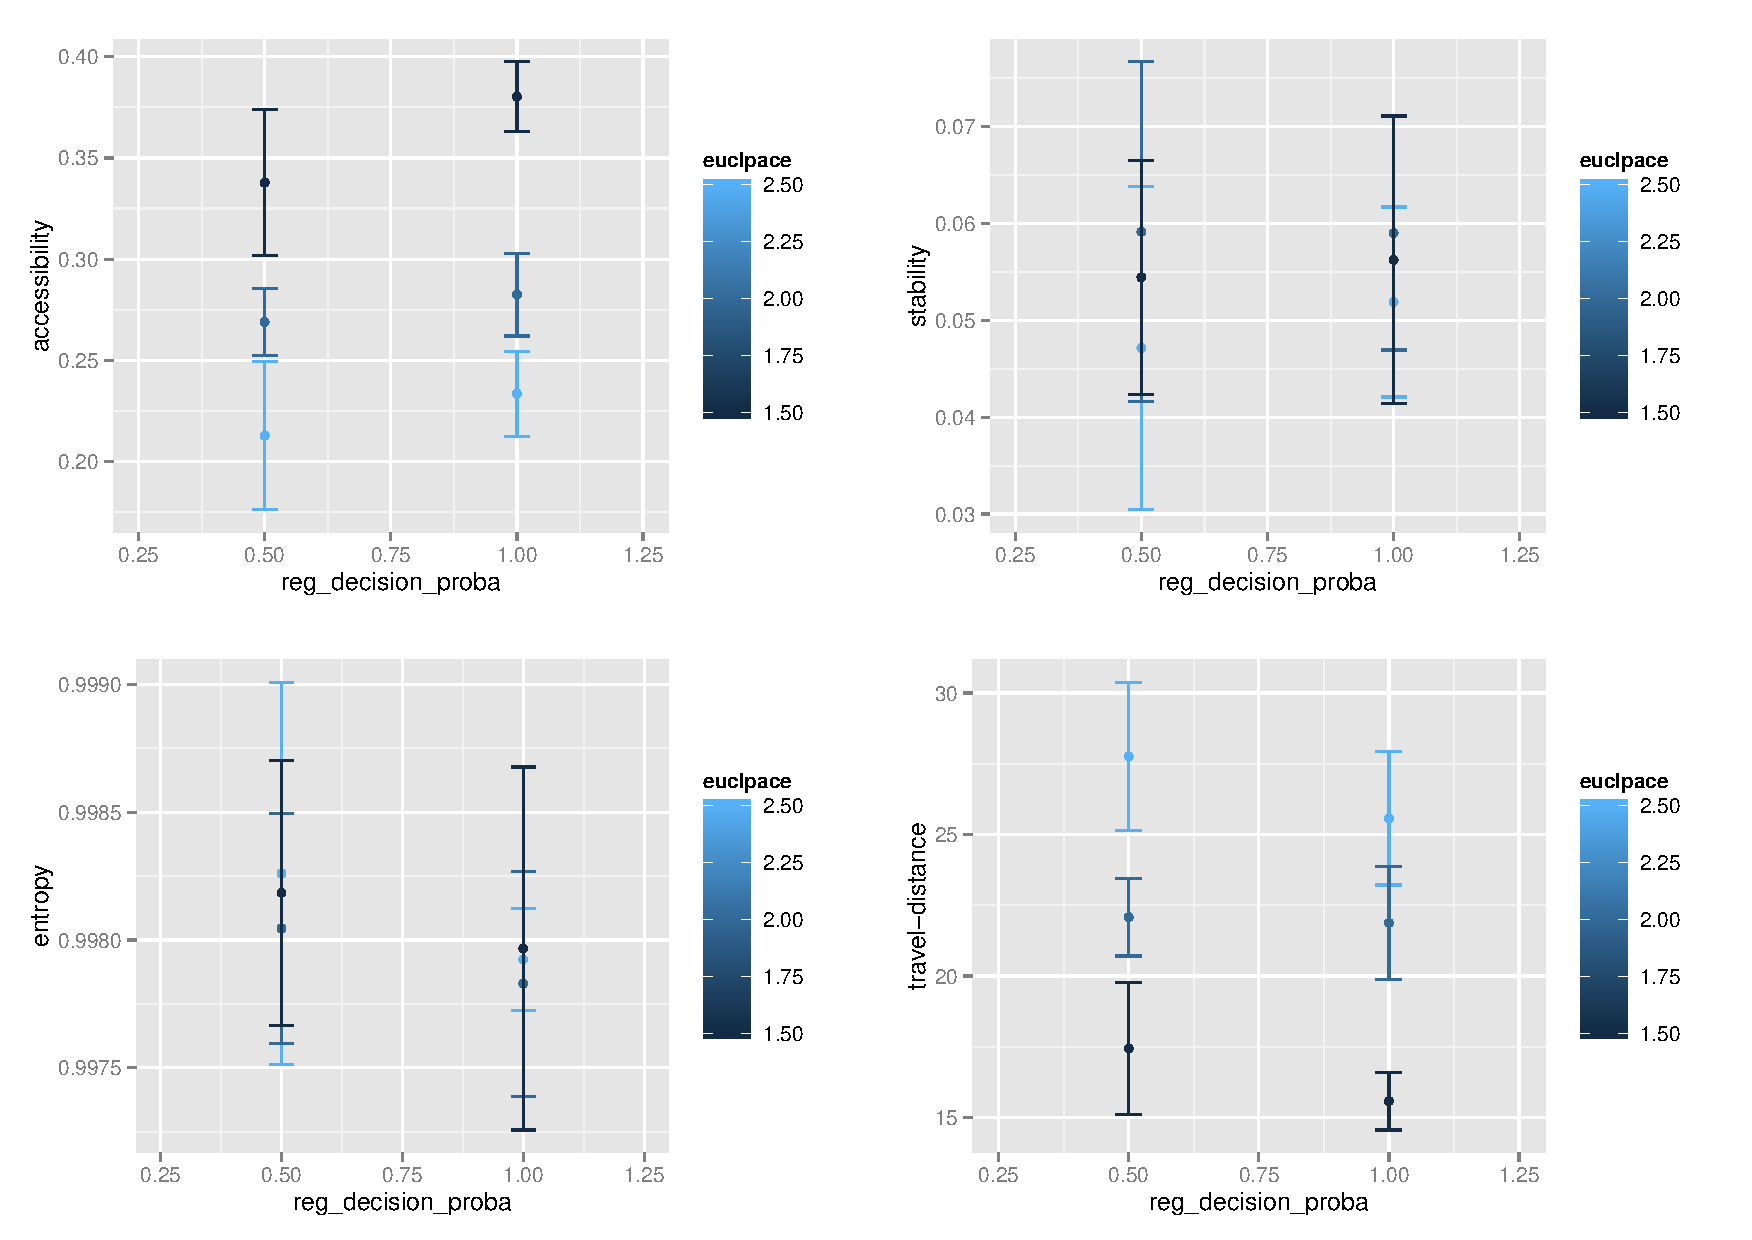
\includegraphics[width=0.6\textwidth,height=0.8\textheight]{figures/allIndics_regProbaVarying_lambdaAcc=0075}

}

%%%%%%%%%%%%%%%%%%%%%%%%%%%%%%%%
\jframe{MetropolSim Model : Next Steps}{
\textit{ -- TBD ASAP, results for ECTQG --}
\bigskip
\begin{itemize}
\item Validation of exploration heuristic on simple urban shapes.
\item Refined exploration heuristic ?
\item Qualitative validation compared to typical luti behaviors.
\item Exploration of various possibilities for gain game matrix.
\item Finer grid exploration.
\item Role of infrastructure speed ; link with the emergence of \emph{megacities}.
\end{itemize}
}





%%%%%%%%%%%%%%%%%%%%%%%%%%%%%%%%
\jframe{Morphological Analysis}{
%\hspace{-1cm}
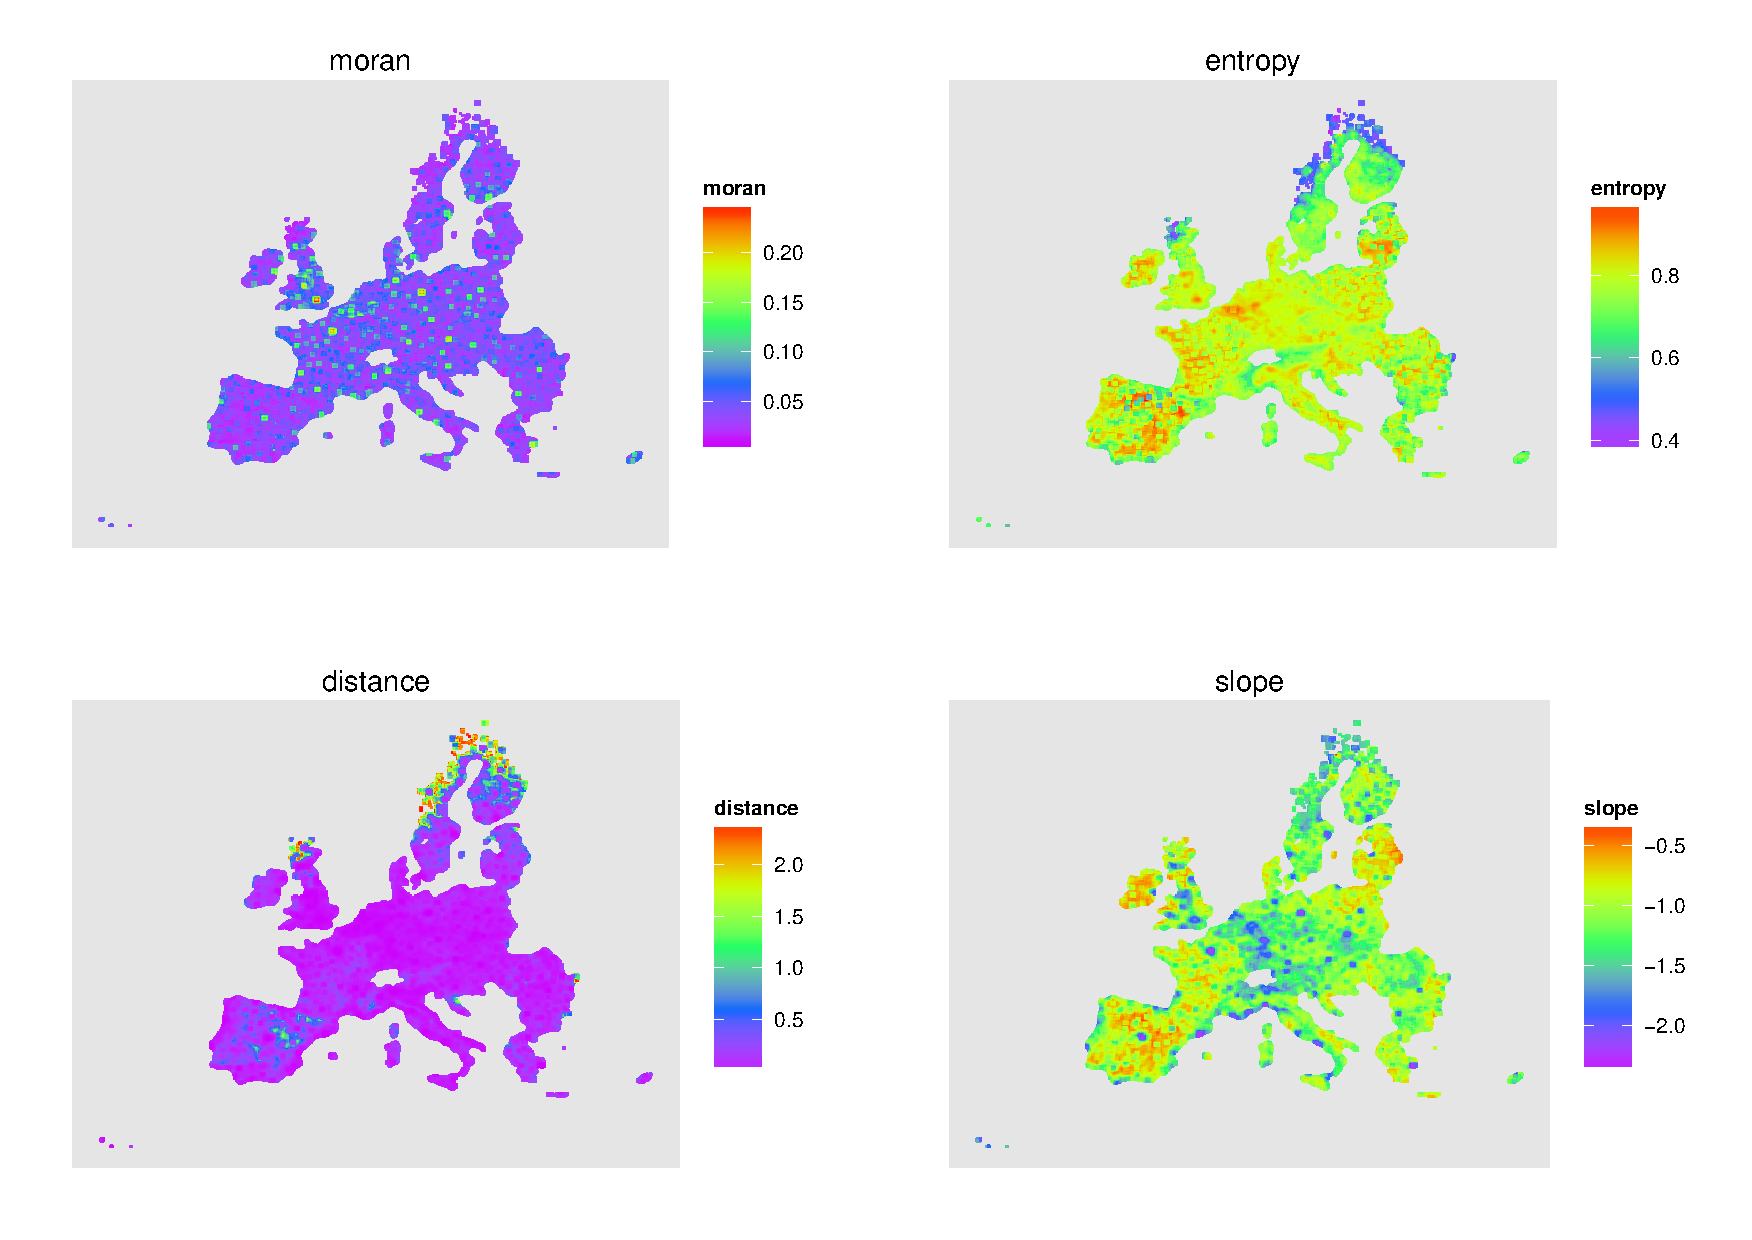
\includegraphics[width=\textwidth,height=0.9\textheight]{figures/all_50km}
}

%%%%%%%%%%%%%%%%%%%%%%%%%%%%%%%%
\jframe{Morphological Analysis : clustering}{
%\hspace{-1cm}
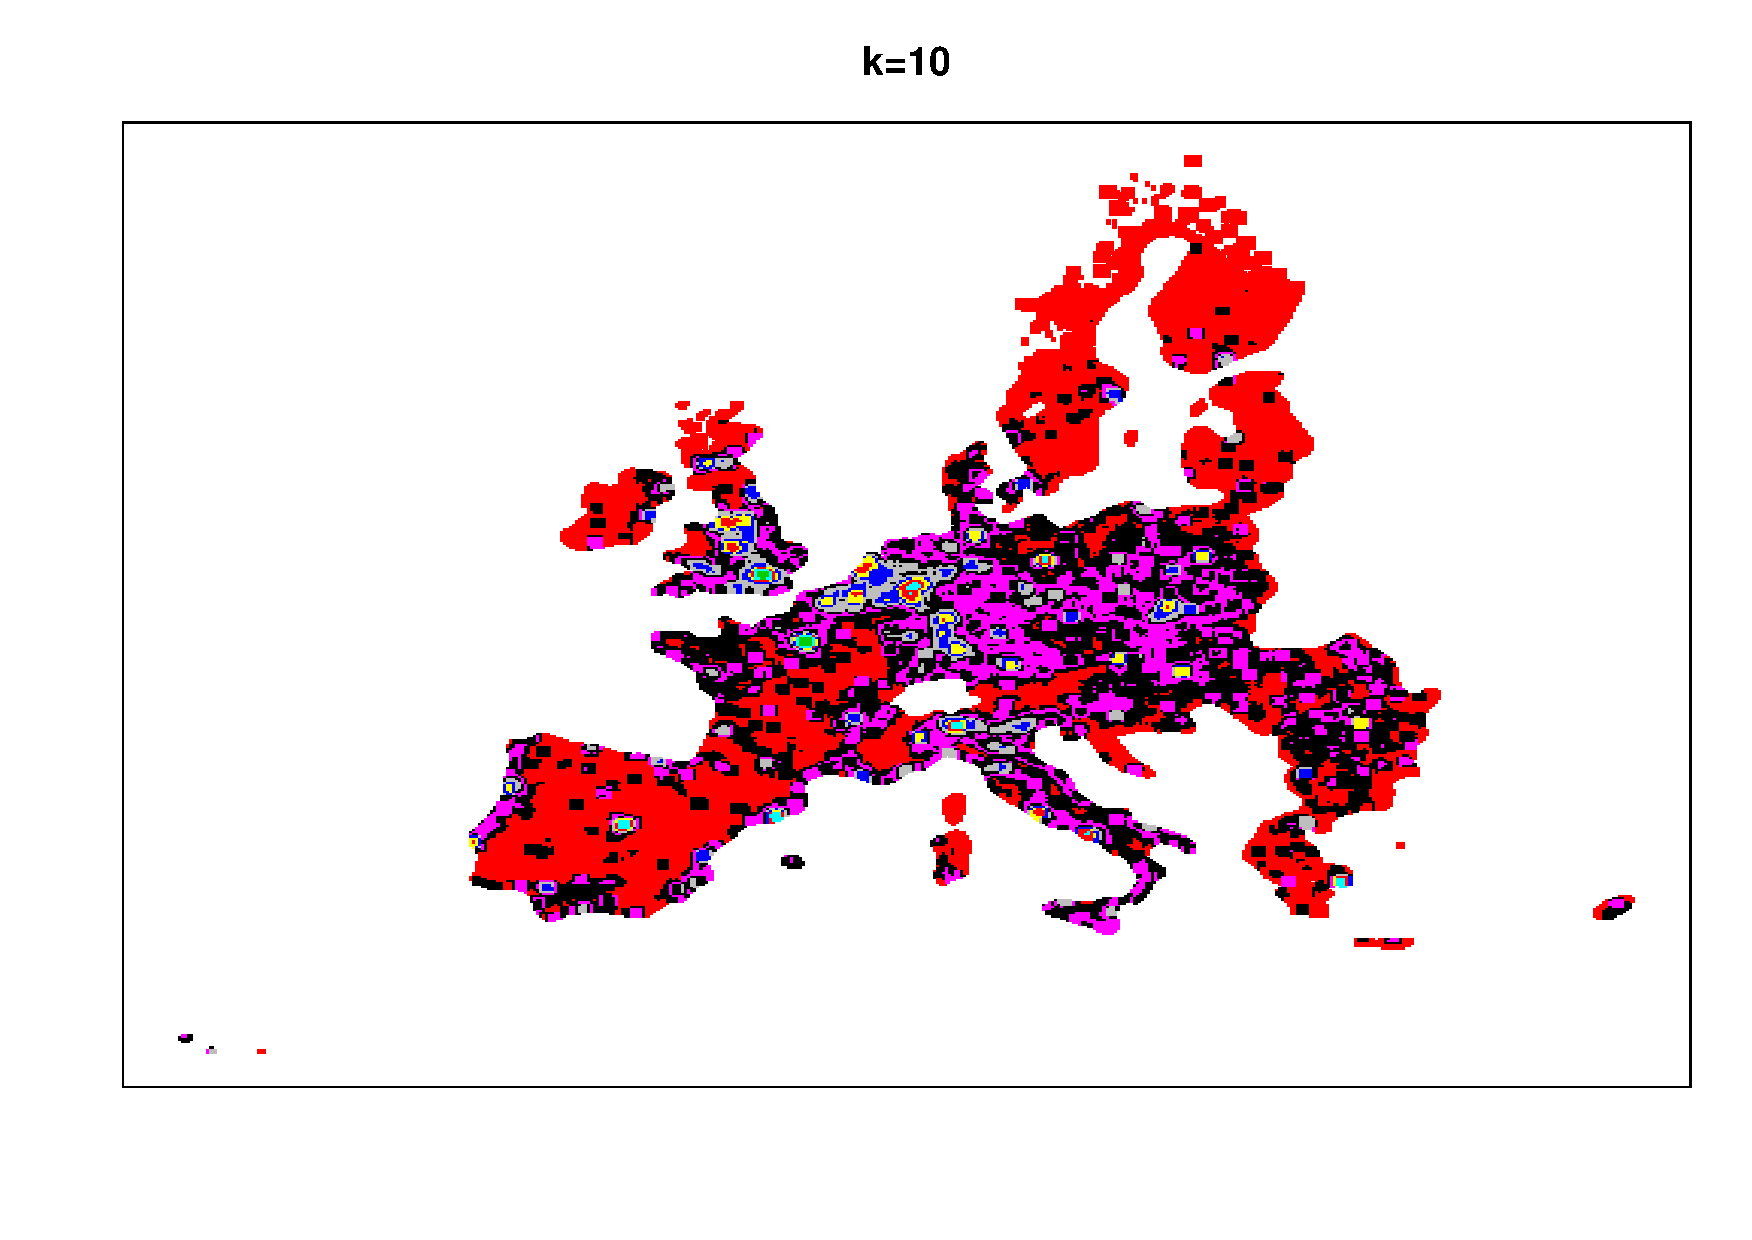
\includegraphics[width=\textwidth,height=0.9\textheight]{figures/cluster_all_k10}
}

%%%%%%%%%%%%%%%%%%%%%%%%%%%%%%%%
\jframe{Morphological Analysis : next steps}{
\begin{itemize}
\item Systematic study of clustering typology, find consistent cluster size reproducing known typology. Test various scales.
\item Analysis on LUZ to validate the method by reproducing Florent results.
\item Network data : street network and railways/public transports directly imported from OSM into R.
\item Network morphological analysis.
\item Coupled statistical analysis of network and urban form, systematically at varying scales [scale is key in our problem].
\end{itemize}
}



%%%%%%%%%%%%%%%%%%%%%%%%%%%%%%%%
\jframe{Synthetic Data Control : On the utility of the approach}{
Context : Model $S$ sensitive to initial conditions $I$, that can be produced by an upstream model $U$. We propose to study the sensitivity of $S$ to $I$ by an exploration of $S\circ U$, allowing statistical control on $U$ parameters (let say $\alpha$) and a better knowledge of the differentiate of $S$.
\medskip
One can object : \textit{Coupling models adds complexity, we do not study the same models. Sensitivity of downstream model can be achieved by the exploration on a large set of $I$.}
\medskip
$\rightarrow$ precisely, one needs quickly a generative model to be able to explore a large number of configurations for $I$.
\medskip
$\rightarrow$ furthermore, even with a dimensionality reduction on $I$ (e.g. morphological classification), one will difficultly know components of its derivative. Whereas studying the coupling allows to know $\partial_{\alpha} I$ and thus $\partial_{I}S$, since $\partial_{\alpha}\left[S\circ U\right] = \partial_{\alpha}S \circ U \times \partial_{\alpha} U$.
\medskip
$\rightarrow$ We also tackle the overall stochastcity, since $\Eb{\Eb{S|I}}=\Eb{S}$.
}


%%%%%%%%%%%%%%%%%%%%%%%%%%%%%%%%
\jframe{Next steps (until August 15th)}{
\begin{itemize}
\item MetropolSim : cf detailed steps. (ETA 1w)
\item Morphology : cf detailed steps. (ETA 1w) ; includes spacematters project.
\item Finish Scaling sensitivity project (ETA 0.4w).
\item Finish Stochastic Urban Growth Framework project (ETA 0.6w)
\item Finish essay (ETA 0.4w)
\item Various tasks (publish nldoc, geoopenmod Banos-Doursat model, literature etc). (ETA 0.6w)
\item Write mid-year memoire / paper (ETA 2w)
\end{itemize}
}




%%%%%%%%%%%%%%%%%%%%%%%%%%%%%%%%
%\begin{frame}[allowframebreaks]
%\frametitle{References}
%\bibliographystyle{apalike}
%\bibliography{/Users/Juste/Documents/ComplexSystems/CityNetwork/Biblio/Bibtex/CityNetwork}
%\end{frame}
%%%%%%%%%%%%%%%%%%%%%%%%%%%%%%%%


\end{document}